\documentclass[10pt]{article}
\usepackage[margin=0.78in]{geometry}
\usepackage{booktabs}
\usepackage{amsmath,amssymb}
\usepackage{microtype}
\usepackage{xcolor}
\usepackage{hyperref}
\usepackage{enumitem}
\usepackage{graphicx}
\usepackage{array}
\usepackage{multirow}
\usepackage{natbib}
\usepackage{tikz}
\usetikzlibrary{arrows.meta,positioning,fit,backgrounds}
\usepackage{tabularx}
\usepackage[most]{tcolorbox}
\usepackage{titlesec}
\usepackage{fancyhdr}
\usepackage{caption}
\usepackage{colortbl}
\hypersetup{colorlinks=true,citecolor=blue,urlcolor=blue,linkcolor=blue}
\definecolor{paperNavy}{HTML}{17324D}
\definecolor{paperTeal}{HTML}{168C80}
\definecolor{paperOrange}{HTML}{D96C24}
\definecolor{paperBlue}{HTML}{2C6EAA}
\definecolor{paperLight}{HTML}{F3F7FA}
\titleformat{\section}{\Large\bfseries\color{paperNavy}}{\thesection}{0.65em}{}
\titleformat{\subsection}{\large\bfseries\color{paperNavy}}{\thesubsection}{0.55em}{}
\captionsetup{font=small,labelfont={bf,color=paperNavy}}
\pagestyle{fancy}
\fancyhf{}
\fancyhead[L]{\scriptsize\color{paperNavy}\textsc{Lazy Distillation}}
\fancyhead[R]{\scriptsize\color{gray}Preliminary controlled study}
\fancyfoot[C]{\thepage}
\renewcommand{\headrulewidth}{0.35pt}
\newtcolorbox{storybox}[1]{
  enhanced,breakable,colback=paperLight,colframe=paperNavy,
  boxrule=0.55pt,arc=2pt,left=6pt,right=6pt,top=5pt,bottom=5pt,
  title={#1},fonttitle=\bfseries,coltitle=white,colbacktitle=paperNavy
}
\newcommand{\takeaway}[1]{%
\begin{tcolorbox}[colback=paperTeal!6,colframe=paperTeal,
  boxrule=0.5pt,arc=2pt,left=5pt,right=5pt,top=3pt,bottom=3pt]
\small\textbf{\color{paperTeal}Takeaway.} #1
\end{tcolorbox}}
\newcommand{\method}{\textsc{LazyDistill}}
\newcommand{\cbias}{\textsc{ConfirmBias}}
\newcommand{\ploss}{\textsc{PatternLoss}}
\newcolumntype{Y}{>{\centering\arraybackslash}p{1.42cm}}

\title{\textbf{When Self-Evolving Agents Learn Too Soon}\\
\large Lazy Distillation Breaks Confirmation-Bias Loops and Preserves Workflow Patterns}
\author{Anonymous preliminary report}
\date{July 2026}

\begin{document}
\maketitle

\begin{abstract}
Self-evolving agents train on experience produced by their own current policy.
Over many train--collect loops, this creates two coupled failures: a wrong
action can become its own training target (\emph{confirmation bias}), and
learning the latest task mixture can erase previously successful workflows
(\emph{pattern loss}).  Existing confidence gates, teacher averaging, and
replay control target quality or memory, but they do not remove the immediate
policy-update$\rightarrow$next-data feedback edge.  We propose \method{}, a
change in learning time: keep the collector frozen for several non-IID waves,
then train once on their pooled evidence.  We construct a controlled benchmark
of 24 confusable tool-use workflows and expose agents for up to 24 repeated
self-evolution cycles.  Simulator oracle actions let us directly measure the
fraction of wrong pseudo-targets, while peak-to-final per-workflow success
measures pattern loss.  At 16 steps and 24 cycles, eager and SDAR-style gated
distillation obtain $0.0\%$ and $3.3\%$ success; \method{} obtains
$79.6\%\pm0.8\%$, reduces pseudo-label error from $95.3\%$ (eager) to
$29.9\%$, and limits pattern loss to $6.4\%$.  The evidence is controlled
rather than a full LLM-agent reproduction, but it identifies update timing as
a causal axis that existing self-distillation objectives leave open.
\end{abstract}

\begin{storybox}{Paper at a glance}
\begin{tabularx}{\textwidth}{>{\bfseries\color{paperNavy}}p{2.05cm}X}
Question & Why do agents that repeatedly learn from their own trajectories
collapse even when each individual update appears reasonable?\\[2pt]
Diagnosis & Eager updates couple two failures: wrong actions become future
targets (\emph{confirmation bias}), while the latest non-IID wave overwrites
previously solved workflows (\emph{pattern loss}).\\[2pt]
Intervention & Freeze the collector across several waves, pool their evidence,
and update once.  This removes within-window error feedback and makes
common/rare patterns co-present during optimization.\\[2pt]
Headline evidence & At 16 steps and 24 cycles, Eager reaches $0.0\%$ success
and SDAR-style gating reaches $3.3\%$; Lazy retains $79.6\%\pm0.8\%$ with
$6.4\%$ pattern loss.
\end{tabularx}
\end{storybox}

\section{Introduction}
\label{sec:introduction}

Self-evolution asks an agent to turn its own interaction history into better
future behavior.  A current policy collects multi-step trajectories, converts
them into pseudo-supervision using feedback or hindsight, updates its
parameters, and repeats.  This paradigm underlies agent self-training methods
such as ReST-meets-ReAct and Re-ReST
\citep{aksitov2023restreact,dou2024rerest}, and recent agentic RL methods such
as SDAR, OPID, and SEED \citep{lu2026sdar,yang2026opid,wu2026seed}.

The long-horizon setting is different from ordinary one-shot
self-distillation because the learner also controls its next training
distribution.  A genuinely self-evolving agent runs
\begin{equation}
 \pi_k \longrightarrow \mathcal{D}_k(\pi_k)
 \longrightarrow \widehat{\mathcal{D}}_k
 \longrightarrow \pi_{k+1},
 \label{eq:loop}
\end{equation}
where the current policy $\pi_k$ determines the trajectory distribution
$\mathcal{D}_k$, and therefore determines its own future supervision.

This closed loop couples two known learning problems into one agent failure.
Pseudo-labeling research calls the first problem \emph{confirmation bias}: an
incorrect model prediction is reused as a label and becomes more confident
\citep{arazo2020confirmation,rodemann2023bayes}.  Continual-learning research
calls the second broad problem \emph{catastrophic forgetting}: later non-IID
updates damage older capabilities \citep{luo2023forgetting}.  We use
\emph{pattern loss} for a precise agent-level measurement of that second
problem: how much full-workflow success falls from its best observed value to
its final value.  Neither term is claimed as new; the new question is why they
reinforce each other over many policy-controlled collection loops.

Existing defenses leave the temporal feedback edge intact.  Confidence
filtering rejects low-confidence labels but fails when the agent is confidently
wrong.  Mean Teacher smooths targets but still updates after each non-IID wave.
Replay retains old examples but may retain old mistakes.  SDAR's positive-gap
gate improves dense token supervision within agentic RL
\citep{lu2026sdar}, yet it also controls loss weight rather than the time at
which a learned policy changes future collection.  Concurrent evidence indeed
finds progressive collapse under multi-iteration agent experience
internalization and favors stable off-policy signals
\citep{chen2026internalization}.

Our solution is to make learning \emph{lazy}, not weak.  As
Figure~\ref{fig:idea} illustrates, \method{} freezes the collector across a
window of different workflow waves and performs one update on their union.
Freezing blocks an early mistake from changing later data in the same window;
pooling makes old, new, common, and rare patterns compete in the same
optimization event.  The method therefore targets the causes of both failures
without requiring an oracle at training time.

\begin{figure}[t]
\centering
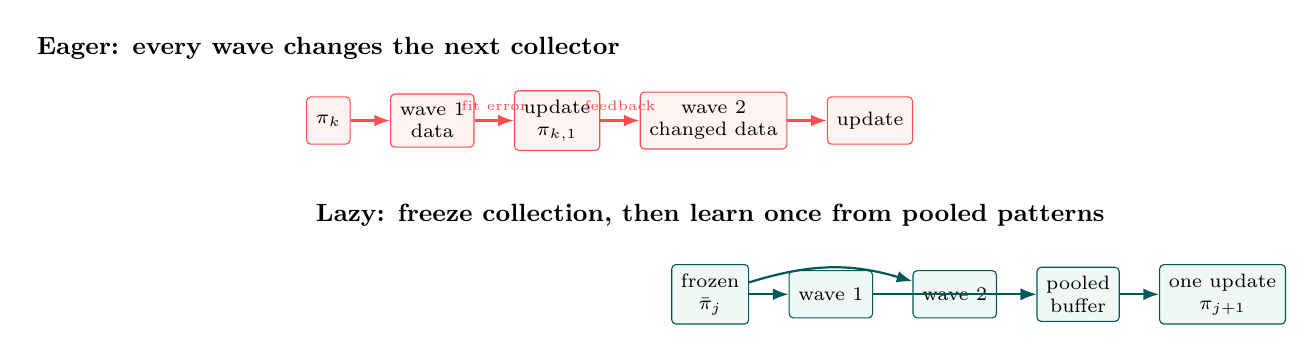
\begin{tikzpicture}[
  node distance=3.5mm and 5mm,
  box/.style={draw,rounded corners=1.5pt,minimum height=6mm,align=center,font=\scriptsize},
  arr/.style={-{Latex[length=2mm]},thick},
  bad/.style={draw=red!70,fill=red!5},
  good/.style={draw=teal!70!black,fill=teal!6}
]
\node[font=\small\bfseries] (eager) {Eager: every wave changes the next collector};
\node[box,bad,below=of eager] (p0) {$\pi_k$};
\node[box,bad,right=of p0] (d1) {wave 1\\data};
\node[box,bad,right=of d1] (p1) {update\\$\pi_{k,1}$};
\node[box,bad,right=of p1] (d2) {wave 2\\changed data};
\node[box,bad,right=of d2] (p2) {update};
\draw[arr,red!70] (p0)--(d1);
\draw[arr,red!70] (d1)-- node[above,font=\tiny]{fit error} (p1);
\draw[arr,red!70] (p1)-- node[above,font=\tiny]{feedback} (d2);
\draw[arr,red!70] (d2)--(p2);

\node[font=\small\bfseries,below=9mm of p0.south west,anchor=west] (lazy)
  {Lazy: freeze collection, then learn once from pooled patterns};
\node[box,good,below=of lazy] (q0) {frozen\\$\bar\pi_j$};
\node[box,good,right=of q0] (b1) {wave 1};
\node[box,good,right=of b1] (b2) {wave 2};
\node[box,good,right=of b2] (pool) {pooled\\buffer};
\node[box,good,right=of pool] (q1) {one update\\$\pi_{j+1}$};
\draw[arr,teal!70!black] (q0)--(b1);
\draw[arr,teal!70!black] (q0) to[bend left=17] (b2);
\draw[arr,teal!70!black] (b1)--(pool);
\draw[arr,teal!70!black] (b2)--(pool);
\draw[arr,teal!70!black] (pool)--(q1);
\end{tikzpicture}
\caption{\textbf{The intervention changes when learning affects future data.}
Eager updates create a short feedback loop; Lazy freezes the collector so
errors cannot alter later waves inside the window, then jointly optimizes all
observed patterns.}
\label{fig:idea}
\end{figure}

Our controlled study makes three contributions.  First, it defines
agent-observable probes that separately measure wrong-target feedback and
workflow erasure.  Second, it provides a procedural long-horizon benchmark in
which the oracle is used only for diagnosis, not training.  Third, across
generic defenses and an SDAR-style gate, it shows that update timing is the
only tested intervention that simultaneously maintains task success, low
pseudo-label error, and low pattern loss.

\section{Related Work and the Missing Axis}

\paragraph{Confirmation bias in self-training.}
Confirmation bias was explicitly studied in deep pseudo-labeling by
\citet{arazo2020confirmation}: incorrect predictions can be selected as labels
and reinforced.  Confidence selection and Bayesian selection reduce exposure
to uncertain targets \citep{radhakrishnan2023enhancing,rodemann2023bayes}.
These methods address which examples enter an update.  In our setting, however,
an error can become highly confident and the update changes which states the
agent visits next; example filtering does not break that temporal edge.

\paragraph{Forgetting under sequential learning.}
Catastrophic forgetting is the degradation of earlier capabilities while
learning later tasks, and it has been observed during continual LLM
fine-tuning \citep{luo2023forgetting}.  Replay and teacher-based consistency
are standard defenses \citep{tarvainen2017mean,yoo2024lpr}, while recent
self-distillation fine-tuning reduces forgetting when learning from
demonstrations \citep{shenfeld2026sdft}.  These methods preserve parameters or
examples.  Pattern loss instead tests an agent-specific outcome---whether a
previously solved multi-step workflow is no longer solved after later
self-generated updates.

\paragraph{Self-improving and self-evolving agents.}
STaR, ReST, ReST-meets-ReAct, and Re-ReST train from generated or repaired
reasoning traces \citep{zelikman2022star,gulcehre2023rest,
aksitov2023restreact,dou2024rerest}.  SDAR uses a privileged-context teacher
and a detached positive-gap gate; OPID and SEED distill hindsight skills from
on-policy trajectories \citep{lu2026sdar,yang2026opid,wu2026seed}.  These
papers improve supervision within an optimization round, but do not isolate
the causal effect of update frequency across many non-IID rounds.  The closest
concurrent work reports multi-iteration capability collapse
\citep{chen2026internalization}; our distinction is a controlled intervention
on update timing plus separate measurements of error reinforcement and
workflow erasure.

\section{Failure Setting}
\label{sec:setting}

The failure can be understood through one concrete tool-use example.  Consider
two visually similar workflows, one requiring
\texttt{search$\rightarrow$open$\rightarrow$extract} and a rarer one requiring
\texttt{search$\rightarrow$filter$\rightarrow$extract}.  If an eager agent
mistakes \texttt{open} for \texttt{filter}, its own pseudo-target may approve
\texttt{open}; the update then makes \texttt{open} more likely in later
collections.  As common examples dominate later waves, the rare
\texttt{filter} workflow can fall from previously solved to consistently
failed.  Confirmation bias describes the wrong target; pattern loss describes
the lost end-to-end workflow.

\begin{storybox}{Running example: one error, two long-horizon consequences}
\begin{tabularx}{\textwidth}{p{1.15cm}Xp{3.6cm}}
\toprule
Time & Event in the self-evolution loop & Diagnostic consequence\\
\midrule
$k$ & Agent chooses wrong \texttt{open}; its pseudo-target copies
\texttt{open}. & A self-reinforced error enters training.\\
$k+1$ & The updated policy visits states caused by \texttt{open} more often. &
Confirmation bias grows across collection rounds.\\
$k+m$ & Common \texttt{open} workflows dominate; rare \texttt{filter}
examples are overwritten. & Previously acquired workflow success is lost.\\
\bottomrule
\end{tabularx}
\end{storybox}

An episode is a partially observed workflow with horizon $H$.  At state $s_t$,
the policy selects one of eight tools.  The hidden workflow program defines the
oracle action $a_t^\star$.  A weak hindsight verifier and the policy distribution
form a pseudo-label:
\begin{equation}
 q_k(a\mid s)=(1-\lambda)\,
 \mathrm{Sharpen}(\pi_k(a\mid s))+\lambda v(a\mid s),\qquad
 \hat a=\arg\max_a q_k(a\mid s).
\end{equation}
The verifier is usually correct but deliberately too weak to override an
already overconfident wrong policy.  This does not force confirmation bias:
it creates the condition under which bias can either grow or be corrected.

\subsection{Probing confirmation bias}

Because the simulator hides an oracle action from the learner, we can diagnose
pseudo-targets without changing training.  We report:
\begin{align}
\mathrm{PseudoErr}_k
 &= \Pr[\hat a_k\neq a^\star],\\
\mathrm{SelfReinforce}_k
 &= \Pr[\arg\max_a\pi_k(a\mid s)\neq a^\star
 \ \wedge\ \hat a_k=\arg\max_a\pi_k(a\mid s)],\\
\mathrm{Amplification}
 &= \mathrm{PseudoErr}_{K}-\mathrm{PseudoErr}_{1}.
\end{align}
We additionally track normalized pseudo-action entropy.  Falling entropy
together with rising self-reinforced error distinguishes collapse from merely
hard data.

In plain language, pseudo-label error asks ``was the training answer wrong?''
and self-reinforcement asks the stricter question ``did the agent copy its own
wrong answer into the training set?''  For example, if the correct tool is
\texttt{search}, the policy chooses \texttt{click}, and the constructed target
is also \texttt{click}, the state counts toward both metrics.  If the verifier
repairs the target to \texttt{search}, it counts toward neither.

\subsection{Probing pattern loss}

Workflows arrive in non-IID waves.  For pattern $p$, let $k_p$ be its first
exposure and $S_{p,k}$ its full-episode success after update $k$.  We define
\begin{equation}
 \mathrm{\ploss}(p)=\max_{k\ge k_p} S_{p,k}-S_{p,K}.
\end{equation}
This asks whether the agent \emph{previously knew} a workflow and lost it after
later self-evolution.  Frozen has zero pattern loss mechanically because it
never updates; it is an ability anchor, not a continual-learning solution.

\begin{table}[t]
\centering
\small
\caption{\textbf{The two pitfalls are measured at different levels.}  Oracle
actions are available to the evaluator only; training receives policy
probabilities and weak verifier feedback.}
\label{tab:metrics}
\begin{tabular}{p{2.5cm}p{5.0cm}p{5.0cm}}
\toprule
Metric & What is counted & What a high value means\\
\midrule
Pseudo-label error &
$\hat a\neq a^\star$, averaged over collected decision states &
The agent is manufacturing incorrect supervision.\\
Self-reinforced error &
The greedy policy action is wrong and the pseudo-label copies that exact action &
The model's own error is directly fed back as a target.\\
Pattern loss &
For each workflow, best post-exposure episode success minus final success &
A workflow was acquired and later erased; this is not merely failure to learn.\\
\bottomrule
\end{tabular}
\end{table}

\section{Lazy Distillation}
\label{sec:method}

\method{} separates collection time from internalization time.  The method has
two deliberately simple modules: a \emph{frozen collection window} that blocks
fast error feedback and a \emph{pooled update} that jointly rehearses every
pattern observed in that window.  For a window of
$W$ non-IID waves, it holds the collector fixed at $\bar\pi_j$:
\begin{equation}
 \mathcal{B}_j=\bigcup_{w=1}^{W}
 \widehat{\mathcal{D}}_{j,w}(\bar\pi_j).
\end{equation}
Only after all waves arrive does it update on the pooled buffer:
\begin{equation}
\pi_{j+1}=\arg\min_\pi
 \sum_{x\in\mathcal{B}_j}
 \ell\!\left(\pi(\cdot\mid s_x),\hat a_x\right).
\end{equation}

\begin{storybox}{LazyDistill in four steps}
\begin{enumerate}[leftmargin=1.5em,itemsep=1pt,topsep=1pt]
\item Snapshot the current agent as the frozen collector $\bar\pi_j$.
\item Collect $W$ non-IID waves with the same $\bar\pi_j$; do not update between
waves.
\item Construct pseudo-targets with policy probabilities and weak verifier
feedback, then pool all waves into $\mathcal{B}_j$.
\item Train once on $\mathcal{B}_j$ to obtain $\pi_{j+1}$ and begin the next
window.
\end{enumerate}
\end{storybox}
\paragraph{Why it targets confirmation bias.}
Within a window, an early wrong update cannot change later trajectories because
there is no within-window update.  The loop gain of
error$\rightarrow$parameter$\rightarrow$data is therefore reduced from every
wave to once per window.

\paragraph{Why it targets pattern loss.}
Common and rare waves are co-present in the same optimization event.  Their
gradients compete jointly instead of the final dominant wave overwriting all
earlier waves.  This is different from replay: replay repairs a sequential
update after it occurs and may repeatedly replay corrupted pseudo-labels.

\section{Experimental Setup}
\label{sec:experiments}

\subsection{Dataset and environment}

We generate 24 procedural workflow patterns organized into 12 confusable
common/rare pairs.  Pair members have highly similar observation cues but
disagree on half of their hidden action programs.  Each observation includes
the workflow cue, current progress, previous tool call, and success/failure
feedback.  Later cycles oversample common patterns, creating a realistic
dominant-trajectory stream without deleting minority patterns.

The main setting uses $H=8$, three attempts per stage, six waves, 12 evolution
cycles, and five seeds.  The scale setting uses $H=16$, 24 evolution cycles,
and three seeds.  Every method starts from the same warm-start policy and sees
the same schedule.  Results report mean and sample standard deviation.

\begin{table}[t]
\centering
\small
\caption{\textbf{Controlled dataset and protocol.}  The scale setting changes
only the two axes central to our hypothesis: episode horizon and number of
self-evolution cycles.}
\label{tab:dataset}
\begin{tabular}{p{4.0cm}ccp{5.0cm}}
\toprule
Property & Main & Scale & Purpose\\
\midrule
Workflow patterns & 24 & 24 & 12 common/rare confusable pairs\\
Actions (tools) & 8 & 8 & Discrete action choice at each state\\
Dependent steps per episode & 8 & 16 & A wrong step changes later observations\\
Attempts allowed per step & 3 & 3 & Environment feedback permits local recovery\\
Non-IID waves per cycle & 6 & 6 & Different pattern subsets arrive sequentially\\
Self-evolution cycles & 12 & 24 & Repeated collect--label--update loops\\
Training tasks per active pattern & 24 & 24 & Identical data budget across methods\\
Evaluation tasks per pattern & 32 & 32 & Full evaluation of all 24 patterns\\
Random seeds & 5 & 3 & Mean and sample standard deviation\\
\bottomrule
\end{tabular}
\end{table}

\paragraph{What one episode looks like.}
A workflow is a hidden length-$H$ program over eight tool actions.  At every
step, the policy observes a 24-dimensional workflow cue, current program
position, previous action, and success/failure feedback.  Confusable pair
members share similar cues but disagree on half of their correct actions.
Thus memorizing the dominant member harms its rare partner.  The full episode
succeeds only if the agent completes all $H$ dependent stages within three
attempts per stage, making the scale setting genuinely long-horizon rather than
16 independent classification examples.

\paragraph{How non-IID evolution is induced.}
Each cycle contains six waves, and each wave activates a subset of patterns.
Later cycles oversample common members while rare members appear less often.
All methods receive the exact same wave order and warm-start state.  This
schedule creates the two necessary stressors without hard-coding failure:
self-generated labels can recursively change, and sequentially dominant
patterns can overwrite rare ones.

\subsection{Comparison methods}

\begin{itemize}[leftmargin=1.4em,itemsep=2pt]
\item \textbf{Frozen}: no parameter updates.
\item \textbf{Eager self-distillation}: update after every wave.
\item \textbf{Confidence-filtered eager}: retain pseudo-labels above a fixed
confidence threshold, following pseudo-label selection defenses
\citep{radhakrishnan2023enhancing,rodemann2023bayes}.
\item \textbf{Mean Teacher}: use an exponential moving-average teacher
\citep{tarvainen2017mean}.
\item \textbf{Eager + replay}: mix each current wave with historical
trajectories, following continual-learning replay
\citep{yoo2024lpr} and growing-batch ReST \citep{gulcehre2023rest}.
\item \textbf{SDAR-style gated eager}: adapt SDAR's detached positive-gap gate
\citep{lu2026sdar} to our action-level policy.  For pseudo-target $\hat a$,
$g=\sigma(\beta[\log q(\hat a\mid s)-\log\pi(\hat a\mid s)])$ is detached and
multiplies cross-entropy.  This isolates SDAR's gating mechanism but is
\emph{not} an exact reproduction of its token-level GRPO system.
\item \textbf{Lazy}: freeze collection for six waves and then
update on all collected pseudo-labels.
\end{itemize}

These implementations isolate the papers' relevant mechanisms; they are not
claimed as exact reproductions on the original datasets.

\section{Preliminary Results}
\label{sec:results}

\begin{storybox}{Evaluation logic}
\begin{tabularx}{\textwidth}{>{\bfseries\color{paperNavy}}p{1.1cm}X}
Q1 & Does repeated eager self-distillation actually create confirmation bias
and pattern loss?\\
Q2 & Do target filtering, teacher smoothing, replay, or delayed timing resolve
both failures?\\
Q3 & Does the distinction persist when both episode horizon and evolution
depth are doubled?
\end{tabularx}
\end{storybox}

\subsection{Does the long self-evolution failure exist?}

Table~\ref{tab:main} first establishes the phenomenon.  Eager
self-distillation collapses from a nonzero frozen policy to zero full-episode
success.  Its pseudo-label error reaches $94.4\%$ on average, and nearly every
wrong greedy action becomes its own target.  Its pseudo-action entropy also
falls, consistent with mode collapse rather than uniformly hard tasks.

\begin{table}[t]
\centering
\scriptsize
\caption{Eight-step, 12-cycle results over five seeds (mean $\pm$ s.d.).
Arrows indicate the preferred direction.}
\label{tab:main}
\begin{tabular}{lYYYY}
\toprule
Method & Success $\uparrow$ & Pseudo error $\downarrow$ &
Self-reinforce $\downarrow$ & Pattern loss $\downarrow$\\
\midrule
Frozen & $35.8\pm5.9$ & $46.4\pm7.1$ & $44.9\pm7.2$ & $0.0\pm0.0$\\
\rowcolor{paperOrange!7}
Eager & $0.0\pm0.0$ & $94.4\pm1.2$ & $94.3\pm1.2$ & $39.6\pm9.7$\\
Confident eager & $54.0\pm30.2$ & $56.8\pm17.2$ & $56.5\pm17.2$ & $26.8\pm14.4$\\
Mean Teacher & $62.8\pm12.9$ & $49.0\pm8.1$ & $48.2\pm8.2$ & $24.3\pm9.3$\\
Eager + replay & $56.6\pm9.3$ & $60.4\pm8.1$ & $60.2\pm8.1$ & $10.5\pm2.6$\\
\rowcolor{paperTeal!10}
Lazy (timing) & $\mathbf{74.0\pm17.8}$ & $\mathbf{43.2\pm12.5}$ &
$\mathbf{43.0\pm12.5}$ & $\mathbf{3.6\pm3.1}$\\
\bottomrule
\end{tabular}
\end{table}

\takeaway{The first experiment establishes the phenomenon before evaluating
the cure: eager learning converts a usable $35.8\%$ frozen policy into a
$0\%$ policy, and $94.3\%$ of collected states directly reinforce the
policy's own wrong action.}

\subsection{Probing whether lazy learning addresses both failures}

The comparison separates three partial defenses.  Confidence filtering is
high-variance because the evolving policy can become confidently wrong.  Mean
Teacher stabilizes targets but still performs sequential non-IID updates.
Replay sharply reduces pattern loss but retains high pseudo-label error because
old incorrect targets are replayed.  Lazy timing is the only updating method in
Table~\ref{tab:main} with both the lowest error feedback and near-zero pattern
loss.  A separate probe found that naively adding a confidence gate to Lazy can
hurt at the longest horizon because the evolving policy becomes confidently
wrong.  This negative result strengthens the timing interpretation: confidence
selection is not a substitute for breaking the recursive update loop.

\subsection{Scale with horizon and evolution depth}

The decisive scale experiment increases both axes that generate the recursive
failure: horizon from 8 to 16 and evolution cycles from 12 to 24.  The final
three-seed values are shown in Table~\ref{tab:scale}.

\begin{table}[t]
\centering
\scriptsize
\caption{Sixteen-step, 24-cycle long-horizon scale experiment.}
\label{tab:scale}
\begin{tabular}{lYYYY}
\toprule
Method & Success $\uparrow$ & Pseudo error $\downarrow$ &
Self-reinforce $\downarrow$ & Pattern loss $\downarrow$\\
\midrule
Frozen & $52.9\pm3.5$ & $24.0\pm3.5$ & $21.9\pm3.5$ & $0.0\pm0.0$\\
\rowcolor{paperOrange!7}
Eager & $0.0\pm0.0$ & $95.3\pm2.5$ & $95.2\pm2.6$ & $19.6\pm8.6$\\
Confident eager & $0.0\pm0.0$ & $93.6\pm1.7$ & $93.5\pm1.7$ & $12.2\pm3.9$\\
Mean Teacher & $79.1\pm9.6$ & $30.3\pm9.1$ & $29.8\pm9.1$ & $11.3\pm4.4$\\
Eager + replay & $24.3\pm4.0$ & $69.4\pm1.6$ & $69.3\pm1.6$ & $10.9\pm7.6$\\
\rowcolor{paperOrange!7}
SDAR-style gate & $3.3\pm3.0$ & $88.3\pm4.0$ & $88.0\pm4.1$ & $41.0\pm15.4$\\
\rowcolor{paperTeal!10}
Lazy & $\mathbf{79.6\pm0.8}$ & $\mathbf{29.9\pm2.9}$ &
$\mathbf{29.8\pm2.9}$ & $\mathbf{6.4\pm4.9}$\\
\bottomrule
\end{tabular}
\end{table}

\takeaway{Difficulty amplifies the distinction.  At twice the horizon and
twice the evolution depth, Lazy and Mean Teacher preserve task ability, but
Lazy retains workflows better; confidence gates, replay, and SDAR-style eager
gating do not jointly control both failure metrics.}

\begin{figure}[t]
\centering
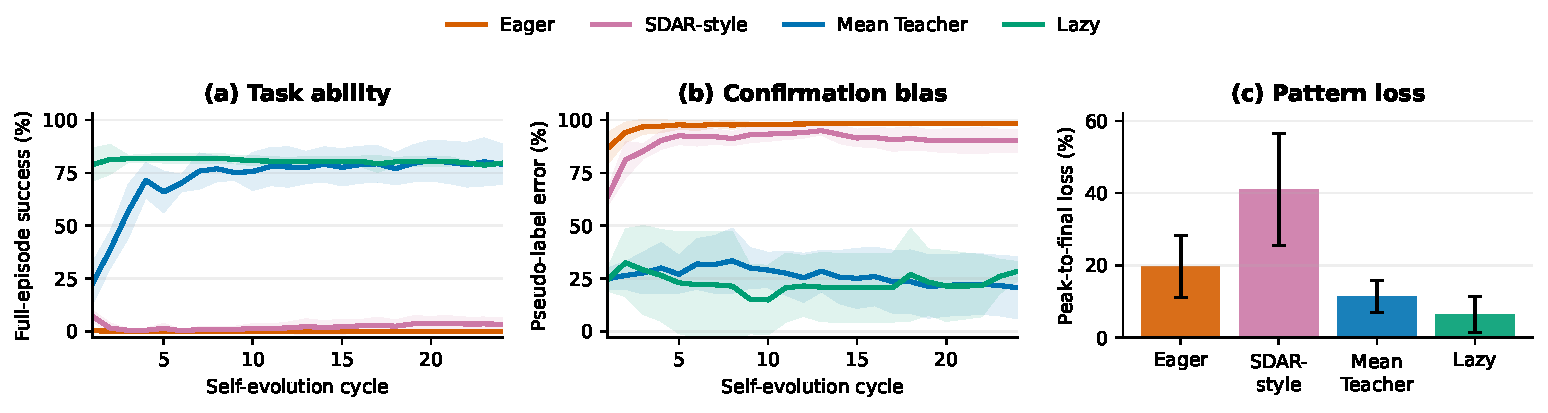
\includegraphics[width=\textwidth]{figures/long_horizon_dynamics.pdf}
\caption{\textbf{Failures emerge over repeated loops, not from one difficult
batch.} Mean $\pm$ one standard deviation across three seeds in the 16-step,
24-cycle setting. Eager and SDAR-style learning rapidly approach near-total
pseudo-label error and lose task ability. Lazy remains stable and has the
lowest pattern loss among updating methods.}
\label{fig:dynamics}
\end{figure}

\subsection{Why SDAR-style gating does not replace lazy timing}

The SDAR-style adaptation reaches only $3.3\%\pm3.0\%$ success and accumulates
$88.3\%\pm4.0\%$ pseudo-label error.  This negative result should not be read
as a leaderboard claim against full SDAR: our controlled policy has neither
language tokens nor GRPO rewards nor a privileged skill-context teacher.
Instead, it is a causal probe of the transferable mechanism.  A positive-gap
gate controls \emph{how strongly} the learner fits each current target, but
eager updates still change the collector after every wave.  Once a wrong
pattern becomes confident, its target can retain substantial weight, affect
later state visitation, and overwrite earlier patterns.

Lazy changes the missing axis: \emph{when} learning is allowed to affect data
collection.  Freezing the collector blocks within-window
error$\rightarrow$data feedback, and pooling all waves makes minority and
majority patterns co-present.  Thus SDAR-style gating and Lazy are conceptually
orthogonal; a full Lazy-SDAR experiment on ALFWorld or WebShop is an important
next step.

\section{Limitations and Next Steps}

This is a procedural stress test with a lightweight policy and a simulator
oracle.  It is designed for causal probing, not external validity.  The
hyperparameter regime was calibrated on one seed before multi-seed evaluation.
The replay baseline receives additional historical examples, so it is
data-reuse matched rather than optimizer-step matched.  Our next experiment
should preserve the same frozen-window intervention in ALFWorld, WebShop, or a
comparable language-agent environment.
The SDAR row is a mechanism adaptation rather than an exact reproduction; a
fair external comparison requires the authors' GRPO stack, language-model
teacher, and original ALFWorld/SearchQA/WebShop protocols.

\section{Conclusion}

Long-horizon self-evolution turns ordinary pseudo-label noise into a dynamical
system: the learner changes the data that will supervise its next version.
Preliminary results show that eager updates can simultaneously amplify wrong
actions and erase old workflows.  Lazy collection attacks the causal link
responsible for the first failure and pooled optimization attacks the sequential
overwrite responsible for the second.  Naive confidence gating is not
sufficient when confidence itself is corrupted.

\bibliographystyle{plainnat}
\bibliography{lazy_distillation}
\end{document}
